\section{Results}
\label{sec:results}

The results of the main project I implemented
during my three-month internship at isMOOD can be divided
into three main categories:

\begin{itemize}
  \item \emph{Phase 1: Research Conduction}: It includes all research that was conducted
  in order to find the most suitable approach
  that would be followed for the accomplishment of the project. 
  \item \emph{Phase 2: Database Construction}: It includes all activities related to the construction
  of the database.
  \item \emph{Phase 3: Algorithm Development}: It summarises all activities related to the development
  of the algorithm in Python.
\end{itemize}

\subsection{Phase 1: Research Conduction}
\label{subsec:research}

To find what approach we would follow,
which are currently the best practices, tools and technologies available
that we would use for the construction of the database
and for the development of the algorithm,
I devoted a two-week time to perform research.

In order to familiarise with the areas
of Text Analytics and Sentiment Analysis,
due to my lack of any previous experience and knowledge on them,
I searched on Google Scholar\footnote{\url {https://scholar.google.gr/}}
for associated research.
At first, my research was not language specific
because my intention was to understand these areas.
Luckily, a variety of studies are publicly available
and I was provided with a lot of information.

From my initial research, I found that 
there are currently two main approaches
to perform Sentiment Analysis in Software Engineering.
The first approach uses Machine Learning methods.
It facilitates from already available data,
however there is one critical restriction.
The algorithm that uses Machine Learning methods
is usually trained on data from specific domains,
thus when a new domain is introduced,
it usually does not perform adequately well.
isMOOD already uses this approach
and is challenged by the abovementioned downside,
and for that reason they asked me to develop
an algorithm based on the second approach
that would be used on untrained domains of data.

The second approach to perform Sentiment Analysis
can be characterised as a more general approach.
It uses a lexicon as its base (lexicon-based)
which contains terms annotated with sentiment,
receives a text as input, divides it into words,
and each word is mapped to the lexicon
in order to find its sentiment.
In its simplest form, the one I also implemented,
the overall sentiment of the text is inferred
through the aggregate-and-average method,
as explained in the thorough guide
to lexicon-based methods for sentiment analysis~\cite{TBTV11};
we sum the sentiment (positive, negative, objective) scores
of all words and divide them with the total number of words.
The preponderant sentiment that occurs in this way
is the final overall text sentiment.

The problem with this approach is that it is language dependent
since it requires a lexicon of terms annotated with sentiment.
From my research, I unfortunately discovered that there are
not enough annotated sources of data for the Greek language.
In order to solve this issue
and generate the required annotated Greek lexicon for our project,
we decided to translate an English annotated lexicon to Greek.

For that purpose I searched and found
that the best publicly available English annotated lexicon
is the SentiWordNet 3.0.\footnote{\url {https://github.com/aesuli/SentiWordNet}}
For the translation, I found that the most appropriate translator
is the Google Cloud Translation API.\footnote{\url {https://cloud.google.com/translate/docs/}}
The downside of Google Cloud Translation API is
that is is not free.
Despite that, when you create a new Google Cloud account
you are currently provided with a free amount of credits
that you can use on any available Google service.
The amount provided was sufficient to translate all terms
included in SentiWordNet 3.0 without being further charged.

For the development of the algorithm,
I was instructed to create a simple algorithm, a baseline.
From the research I conducted and after a lot of fruitful discussions
with all the professionals mentioned
in Section~\ref{subsec:technical-activities},
I decided to use lemmatisation on words that were not directly mapped
to the Greek annotated lexicon,
and then use the average-and-aggregate method
for the calculation of the overall text sentiment.
For the lemmatisation, I discovered
that the best available lemmatiser in Python
adapted to the Greek language is provided
by the spaCy library.\footnote{\url {https://spacy.io/models/el#el_core_news_md}}

\subsection{Phase 2: Database Construction}
\label{subsec:database}

The most time consuming process of the project
was the construction of the database that would be used;
this process took almost two months.
There are three main reasons for that.

The first reason lies in the multiple reconstructions
that I made to the database schema;
the schema changed more than five times.
What I learned and what my supervisor informed me is
that as you build a database,
the schema matures in your mind,
and as you process the information stored,
you find more efficient ways to represent it in the database.

The second reason lies in the time consuming queries
that I had to run in order to store all information.
All queries to the MongoDB database were run through OpenVPN
on a 6-core Cloud Virtual Machine with 16GB RAM
provided by DigitalOcean.
The queries were executed far more quickly in this way
than on a local computer, plus I could run them
in screen mode and have parallel executions of multiple queries,
without worrying about any interruptions
that would lead to the failure of a query.

Despite that, some queries would run for days.
For instance, the population of the Greek lexicon with the lemmas
produced from it took five days.
Furthermore, the sentiment mapping from the translated terms
of SentiWordNet 3.0. to the terms of the Greek lexicon
required two days.
What is more, some time consuming queries, like the sentiment mapping,
had to be executed repeatedly as the database schema changed,
in order to ensure consistency and validity for the data.

In addition,
the fact that the Technical team made urgent changes and updates
to the MongoDB that required for the MongoDB to be restarted immediately
while some of my queries were executed at the same time,
would lead to the untimely termination of them.
Some of them were not possible to continue
from the point they had stopped,
thus had to run from the beginning again.

The third reason behind the time consuming construction of the database
is related to the complex information that was stored.
A lot of sources were used and combined to gather information,
and multiple processes were performed on them
to transform the information in the desired format
and then produce extra attributes.

At the end, the final database schema in MongoDB
that we named ``lexicondb''
is composed of four collections,
as depicted in the following figure,
and they are all explained in detail.
Statistics of the collections are also included,
along with an example of a record.

\begin{figure}[ht]
\centering
\includegraphics[width=\textwidth]{mongodb-schema.eps}
\caption{MongoDB Database Schema -- lexicondb}
\label{fig:mongodb-schema}
\end{figure}

\clearpage

\subsubsection{swn\_v3}
\label{subsubsec:swn-v3}

This is the first collection that was created.
It contains all records of SentiWordNet 3.0.
The data of the source file that is publicly available\footnote{\url {https://github.com/aesuli/SentiWordNet/blob/master/data/SentiWordNet_3.0.0.txt}}
and that was used are in a complex format,
making it the most difficult data source that had to be parsed
for the construction of the particular database.
The source file was initially converted
from text (txt) format to comma-separated-values (csv) format,
and all comments included in the file were removed
to make it parsable.

While parsing it with a Python script, it was discovered that
some fields do not always follow a standard pattern.
All troubled fields were manually inspected
in order to detect all possible patterns that were followed.
Then multiple checks and filters were applied to the Python script 
according to the detected patterns,
in order to construct the particular collection,
based on a standard format.
We finally formed the following fields:

\begin{itemize}
  \item \emph{\_id}: A concatenation of the ``pos'' (part-of-speech)
  and the ``id'' fields of the source file.
  This is the unique id of each record according to the SentiWordNet 3.0
  documentation provided in the beginning of the source file. 
  
  \item \emph{sentiment}: It includes the fields ``PosScore'' (Positive Score)
  and ``NegScore'' (Negative Score).
  The field ``ObjScore'' (Objective Score) is calculated
  based on the following formula according to the documentation: \\
  $ObjScore = 1 - (PosScore + NegScore)$
  
  \item \emph{gloss}: The most troubled field.
  It includes explanations and examples of the use of the synonym sets
  of the particular record.

  For the examples, we noticed that they start with quotation marks
  and initially distinguished them based on that.
  We later found that some examples also include other phrases 
  in quotation within them (e.g. ``the word `dog' is animate'')
  and this was not initially covered by our filters,
  leading in some cases to wrong inputs to the field ``examples''.
  In the above example, there would be inserted three examples
  instead of one: ``the word'', ``dog'', ``is animate''.
  We fixed this by applying regex rules
  that bypassed the inside quotation marks.

  For the explanations, we simply checked for a phrase
  whether it was an example according to the above rules,
  and if not, then is was an explanation.
  All phrases are separated by a semicolon (``;'')
  and we used this as a delimiter to separate the phrases
  of each record.
  We also included the number of explanations and examples
  found in the particular record.
  
  \item \emph{pos}: The part-of-speech of the record.
  
  \item \emph{synsets}: One major difference between SentiWordNet 3.0
  and 1.0 (the previous version) is
  that 3.0 follows the ``bag-of-synsets'' logic
  instead of ``bag-of-words'' that is followed in 1.0~\cite{BES10}.
  This means that each record contains multiple terms
  that are semantically associated (synonym sets).
  
  For each record, we separated all terms included,
  and made an object for each term under ``synsets''.
  Each ``term'' contains a ``sense\_number'' from the source file,
  which is a number that indicates the relevance of the term
  to the particular synonym set, starting with a hashtag (``\#'').
  In addition, we used spaCy library
  to derive more grammatical information~\footnote{\url {https://spacy.io/usage/linguistic-features}}
  about each term, and placed it under the field ``spacy''.
  
  \item \emph{swn\_id}: The id included in the source file for each record.
  However, this id is not unique.
  
  \item \emph{synsets\_count}: The number of terms
  found in the particular synonym set.
\end{itemize}

\subsubsection{english\_sentiment\_terms}
\label{subsubsec:english-sentiment-terms}

After constructing swn\_v3,
we constructed a second collection
with the unique terms found in SentiWordNet 3.0 as ids.
What was noticed is that some terms are included
in multiple synonym sets;
for these, the sentiment scores are averages
(the scores of all occurrences of a term were summed
and divided with the number of occurrences).
The fields included in this collection are the following:

\begin{itemize}
 \item \emph{\_id}: A unique term of swn\_v3.

 \item \emph{sentiment}: It contains the average sentiment scores
 (``PosScore'', ``NegScore'', ``ObjScore'') computed as described above.
 It also includes the preponderant sentiment based on the maximum score
 (field ``majority'').

 ``magic\_number'' is a number that occurred after a lot of hours
 of discussion with my colleagues of the Technical team.
 We wanted to produce a number that would indicate for a term
 how strongly annotated it is
 (i.e. how much difference there is among its sentiment scores).
 At the end, we came up with the following formula: \\
 $magic\_number = (max\_score - intermediate\_score) + (max\_score - min\_score)$ \\
 This number receives values in range $[0,2]$.
 
 \item \emph{sources}: It includes all ids of the swn\_v3 records
 where the particular term was found.
 
 \item \emph{sources\_count}: The number of the above record ids.
 
 \item \emph{translation}: The translation of the term in Greek
 based on the Google Cloud Translation API
 as described in Section~\ref{subsec:research}.
 Two versions of the translation are included:
 the raw translation and the translation in lowercase.
 The second is used to match a translation of an English term
 to a Greek term of greek\_terms in order to transfer sentiment,
 excluding any case sensitivity.
 
 \item \emph{words\_count}: Some terms are phrases, thus
 it is listed for each term how many words it is composed of.
\end{itemize}

\subsubsection{greek\_terms}
\label{subsubsec:greek-terms}

For the creation of the Greek lexicon,
three initial data sources were used:

\begin{enumerate}
 \item \emph{Aspell}: An official Greek dictionary used in OpenOffice/LibreOffice Spell~\footnote{\url {http://www.elspell.gr/myspell}}
 that contains 828,806 terms.
    
 \item \emph{Wiktionary}: A dictionary of 92,747 Greek terms from Wiktionary.~\footnote{\url {https://github.com/eellak/gsoc2018-spacy/blob/6212c56f94ca3926b0959ddf9cee39df28e1c5a8/spacy/lang/el/lemmas/elwords_from_wiktionary.txt}}

 \item \emph{Hunspell}: A collection of 458,331 Greek terms from Hunspell.~\footnote{\url {https://github.com/eellak/gsoc2018-3gm/blob/master/resources/greek_lemmas.py}}
\end{enumerate}

The dictionary was then populated with the lemmas of the terms
derived from spaCy library, leading to 97,793 new records in the collection.
Eventually the following fields were constructed:

\begin{itemize}
 \item \emph{\_id}: A unique term derived from one of the above data sources.
 
 \item \emph{clean}: The term in lowercase with no accentuation.
 
 \item \emph{sentiment}: The sentiment mapped from english\_sentiment\_terms
 based on the lowercase translation.
 If the term was found in multiple lowercase translations,
 then the average scores are computed and inserted.
 The preponderant sentiment that corresponds to the maximum sentiment score
 is also included, along with the magic number as described before.
 
 \item \emph{sources}: The data source(s) of the term:
 ``aspell'', ``wiktionary'', ``hunspell'', ``lemmas\_generated''.
 
 \item \emph{sources\_count}: The number of data sources of the term.
 
 \item \emph{spacy} Grammatical information of the term
 derived from spaCy library.
 
 \item \emph{words\_count}: The number of words that the term is composed of.
\end{itemize}

\subsubsection{greek\_sentiment\_terms}
\label{subsubsec:greek-sentiment-terms}

The last collection that was created
contains the clean terms of greek\_terms as ids.
The reason lies in the algorithm,
as described in Section~\ref{subsec:algorithm};
the input text is cleaned from any case sensitivity or accentuation,
thus a clean version of the Greek lexicon was needed
in order to match the words of the input text to the words of the lexicon.

This collection contains only words ($words\_count = 1$)
that have received sentiment through the process
described in Section~\ref{subsubsec:greek-terms}.
If a clean word was found in multiple records of greek\_terms,
again the average scores are computed and inserted
to the ``sentiment'' field.
The fields of this collection are listed below:

\begin{itemize}
 \item \emph{\_id}: A unique clean term from greek\_terms.
 
 \item \emph{pos}: The part-of-speech of the term.
 In cases of multiple occurrences of a clean term in greek\_terms,
 the part-of-speech receives the preponderant value,
 by counting the frequences of each part-of-speech
 and computing the maximum value.
 
 \item \emph{sentiment}: The sentiment of the clean term.
 Again in multiple occurrences of the clean term,
 the average scores are computed and inserted.
 
 \item \emph{sources\_count}: The number of occurrences
 of the clean term in greek\_terms.
 
 \item \emph{words\_count}: Since only single words are included,
 this field always has the value ``1''.
\end{itemize}

\subsubsection{Statistics}
\label{subsubsec:statistics}

The number of records of each collection is listed below:

\begin{itemize}
 \item \emph{swn\_v3}: 117,659 records
 \item \emph{english\_sentiment\_terms}: 148,834 records
 \begin{itemize}
  \item 4,869 with positive preponderant sentiment
  \item 7,269 with negative preponderant sentiment
  \item 136,696 with objective preponderant sentiment
 \end{itemize}
 \item \emph{greek\_terms}: 951,755 records
 \begin{itemize}
  \item 132,943 only from Aspell
  \item 6,399 only from Wiktionary
  \item 55 only from Hunspell
  \item 97,793 new terms (lemmas) produced from spaCy library
  \item 427,233 from two sources
  \item 271,124 from three sources
  \item 16,208 from four sources
 \end{itemize}
 \item \emph{greek\_sentiment\_terms}: 27,542 records
 \begin{itemize}
  \item 1,252 with positive preponderant sentiment
  \item 1,883 with negative preponderant sentiment
  \item 24,407 with objective preponderant sentiment
 \end{itemize} 
\end{itemize}

To the best of our knowledge,
the collection ``greek\_sentiment\_terms'' currently forms
the largest publicly available Greek lexicon annotated with sentiment.

\subsubsection{Example of Record}
\label{subsubsec:example}

In the following figures
the Greek term ``\textgreek{kakos}'' occurred in greek\_sentiment\_terms
from the term ``\textgreek{kak'os}'' of greek\_terms.
The terms ``maleficent'' and ``wicked'' of english\_sentiment\_terms
are translated as ``\textgreek{kak'os}''.
``maleficent'' was found in one record in swn\_v3,
whereas ``wicked'' was found in five records. \\

\textbf{greek\_sentiment\_terms: \textgreek{kakos}} \\

\begin{center}
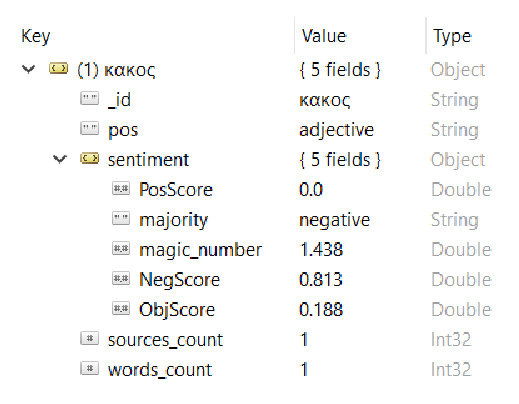
\includegraphics{record/greek-sentiment-terms-kakos.eps}
\end{center}

\clearpage

\textbf{greek\_terms: \textgreek{kak'os}} \\

\begin{center}
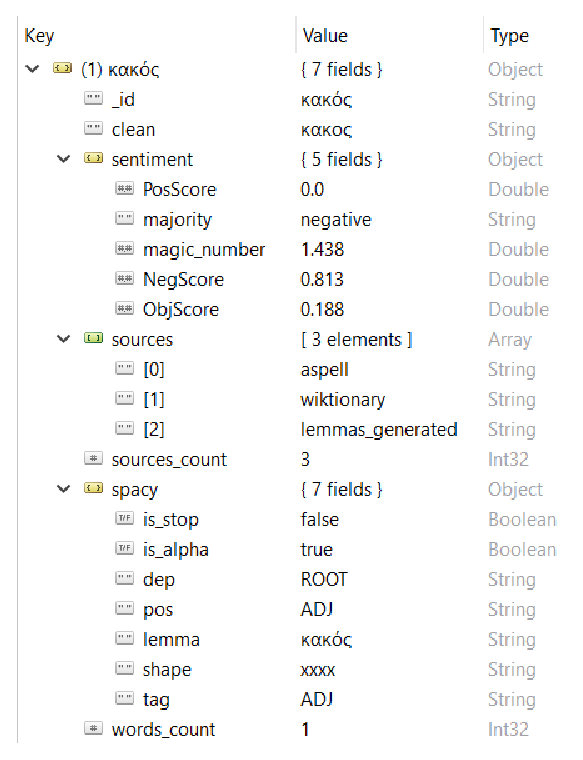
\includegraphics{record/greek-terms-kakos.eps}
\end{center}

\clearpage

\textbf{english\_sentiment\_terms: maleficent} \\

\begin{center}
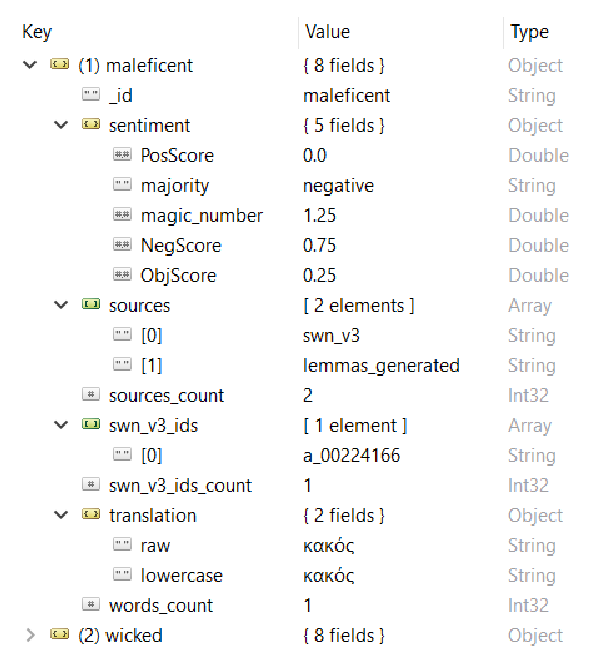
\includegraphics{record/english-sentiment-terms-maleficent.eps}
\end{center}

\clearpage

\textbf{english\_sentiment\_terms: wicked} \\

\begin{center}
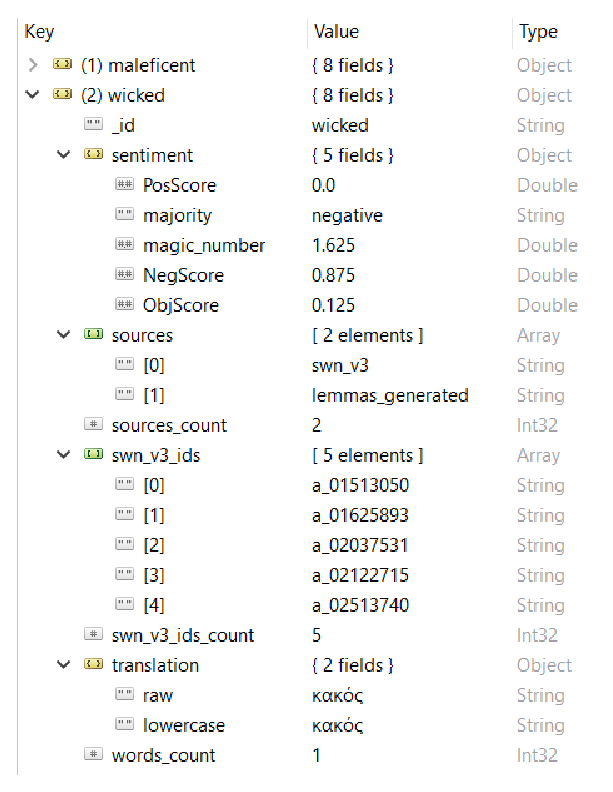
\includegraphics{record/english-sentiment-terms-wicked.eps}
\end{center}

\clearpage

\textbf{swn\_v3: maleficent} \\

\begin{center}
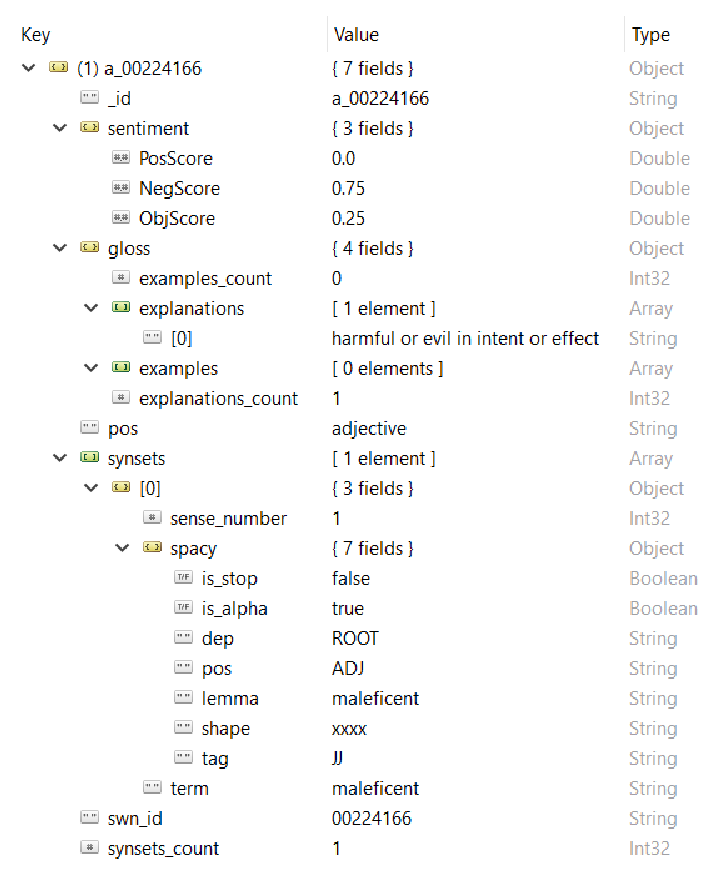
\includegraphics{record/swn-v3-maleficent.eps}
\end{center}

\clearpage

\textbf{swn\_v3: wicked} \\

\begin{center}
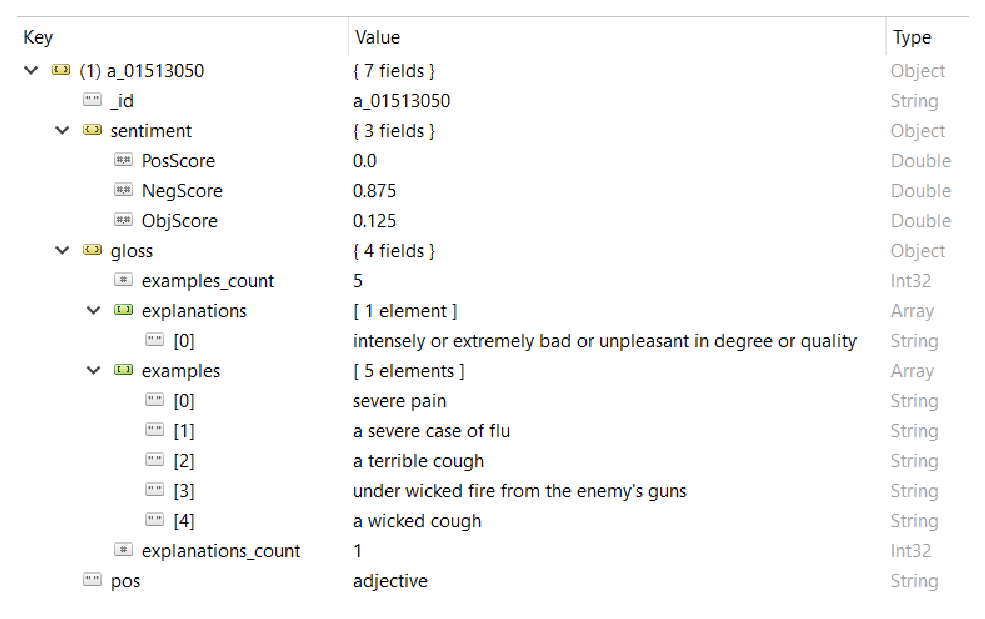
\includegraphics{record/swn-v3-wicked.eps}
\end{center}

\clearpage

\textbf{swn\_v3: wicked} \textit{(continues)} \\

\begin{center}
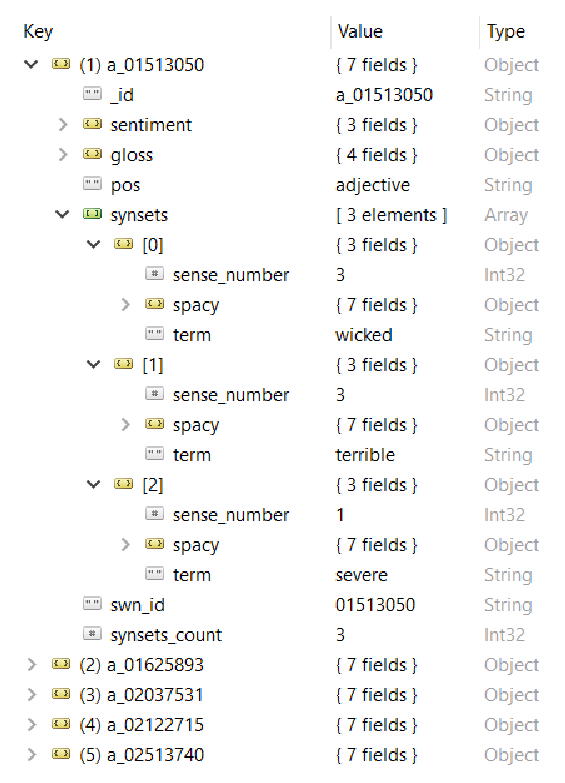
\includegraphics{record/swn-v3-wicked(2).eps}
\end{center}

\clearpage

\subsection{Phase 3: Algorithm Development}
\label{subsec:algorithm}
